\section{Further Analysis and Discussion}
\label{sec:analysis}

% This section analyzes how private agents behave when collaborating under privacy constraints.
% We analyze the interaction dynamics between task completion and privacy constraints to characterize systematic behaviors and failure modes.
To systematically study collaboration among private agents under privacy constraints, we organize our evaluation around the following research questions:
% \newline\textbf{RQ1:} \textit{Can multi-agent collaborate under privacy constraints?} 
\newline\textbf{RQ1:} \textit{Does collaboration differ between single private-agent and dual private-agent?}
\newline\textbf{RQ2:} \textit{Does collaborative task performance remain consistent across different agent pairings?}
\newline\textbf{RQ3:} \textit{Which kinds of privacy constraints make it challenging to simultaneously achieve high $\mathbf{Acc}_{\mathbf{joint}}$?}

% \subsection{(RQ1) Effects of Privacy Constraints on Collaborative Outcomes}
% \label{sec:analysis_RQ1}

% We first examine how explicit privacy constraints reshape collaborative outcomes. 
% While agents are often able to make partial task progress, our analysis reveals systematic tensions between task advancement and privacy compliance that emerge during interaction.

% \paragraph{Task–Privacy Trade-offs.}
% \label{sec:privacy_task_trade_off}

% Figure~\ref{fig:experiment_0vsOther} contrasts task performance between episodes with no privacy compliance (PS~=~0) and those achieving at least partial privacy compliance (PS~$>$~0). 
% For GPT-5.1 and Claude, enforcing privacy constraints leads to a clear reduction in task success, indicating a direct tension between task progress and privacy preservation. 
% In contrast, LLaMA and Qwen exhibit a slight increase in task performance when privacy constraints are satisfied. 
% This suggests that, for some models, privacy constraints may act as a form of regularization, encouraging more cautious and structured information exchange. 



% \input{figures/figure5}


% task 종료가 홀수 턴에만 이루어짐 -> 이걸 통한 분석 쓰기 (GPT 추천. 주도권으로 분석 쓰기)
\subsection{RQ1. Single vs. Dual Private-Agent Collaboration}
\label{sec:analysis_RQ1}

While privacy constraints are present in both the single and dual-private-agent settings, they differ in how these constraints are distributed across agents. 
Therefore, we examine how this difference shapes collaboration dynamics, solely focusing on agent roles and coordination patterns (Table~\ref{tab:privacy_success}).
% rather than task performance.


\paragraph{Asymmetric interaction roles in single-private settings.}
\label{sec:asymmetric_roles}

To characterize role asymmetry in single-private settings, we measure the presence of questions in agent messages, using question frequency as an observable proxy for information-seeking behavior. 
We focus on settings where privacy constraints are applied to only one agent (Agent A).

\begin{table}[H]
\centering
\small
\begin{tabular}{lcc}
\toprule
\textbf{Setting} & \textbf{Agent} & \textbf{Question Rate} \\
\midrule
\multirow{2}{*}{Single Agent} 
 & Private Agent & 58.08\% \\
 & Non-Private Agent & 0.00\% \\
\midrule
\multirow{2}{*}{Dual Agent} 
 & Initiate Private Agent & 54.22\% \\
 & Partner Private Agent & 50.61\% \\
\bottomrule
\end{tabular}
\caption{Rates of messages containing questions under single private agent and dual private agent settings.}
\label{tab:privacy_success}
\end{table}


Our results reveal a striking role asymmetry. 
All question-containing messages are produced by the private agent, while the non-private agent (Agent B) asks no questions at all. 
This behavior suggests that privacy ownership fundamentally restructures collaborative dynamics. 
Instead of bidirectional information seeking, single-private interactions exhibit a one-sided structure in which the private agent probes for information and the non-private agent responds.
These findings demonstrate that privacy constraints shape not only what information is shared, but also who drives the interaction.

\paragraph{Coordination slowdown under dual-private constraints.}
\label{sec:dual_private_slowdown}

We analyze coordination efficiency by measuring the turn at which each task requirement is satisfied.
Compared to single-private settings, dual-private collaboration shows a clear coordination slowdown: requirements are resolved over a wider range of turns, and a substantial fraction remain unsatisfied by the end of the interaction.
This pattern indicates higher coordination costs under mutual privacy constraints, where limited information exchange leads to slower and sometimes incomplete convergence.


\subsection{RQ2. Effects of Partner on Private-Agent Collaboration}
\label{sec:analysis_RQ2}
 
Using a holistic success metric that jointly evaluates task completion and privacy compliance, we analyze how partner intent influences collaboration outcomes.

\begin{figure}[t]
    \centering
    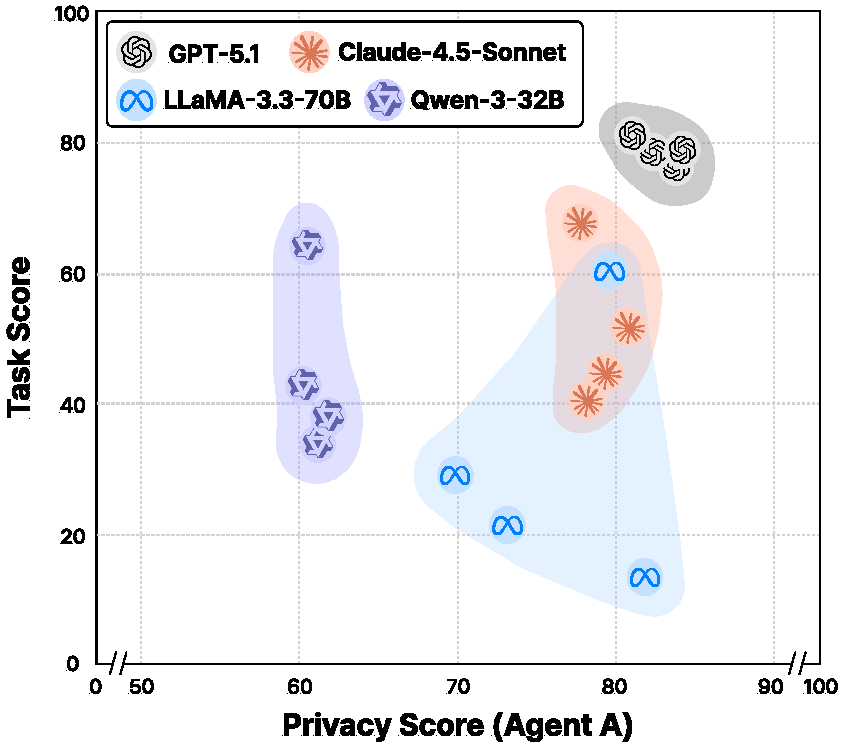
\includegraphics[width=\columnwidth]{images/figure_5_camready.pdf}
    \caption{Model-level distributions in the task--privacy space. GPT consistently occupies a stable high-performance region across different partner models, whereas other models exhibit larger variability depending on their collaborators.}
    \label{fig:model_performance}
\end{figure}

\paragraph{Consistent performance anchor via solution priming.}
As shown in Figure~\ref{fig:model_performance}, GPT-5.1 consistently exhibits strong joint performance across different partner models, maintaining high $\mathbf{Acc}_{\mathbf{joint}}$ while other models show greater performance variance depending on their counterparts. 
Qualitative analysis suggests that this robustness arises from a tendency to proactively introduce new criteria or solution strategies at the early stage of collaboration.
By reframing the task and establishing a clearer solution structure, the model implicitly guides coordination with the partner model, thereby stabilizing joint performance even when collaborating with models of varying capabilities.


\paragraph{Holistic performance degradation under adversarial partners.}

Across all evaluated settings, collaboration with adversarial partners consistently results in lower holistic success rates compared to cooperative settings. This degradation is observed across models and privacy configurations, indicating that adversarial behavior systematically undermines joint task--privacy success. 
Detailed results across cooperative and adversarial partner settings across models are provided in Appendix~\ref{app:holistic_partner_results}.



\subsection{RQ3. Effects of Different Privacy Constraints on $\mathbf{Acc}_{\mathbf{joint}}$}

In private-agent collaboration, agents contribute to joint reasoning through their own private information, making privacy constraints a key factor that shapes coordination. 
We categorize privacy constraints into two types: (i) \emph{range-based privacy}, which prohibits disclosing any specific subset of the underlying data distribution and (ii) \emph{change-based privacy}, which prohibits reproducing the original sensitive value.

\paragraph{Range-based privacy.}
Range-based privacy violations arise when an agent reveals information about a specific subset of its private data, such as a particular segment or category. 
Although agents avoid direct disclosure of the original value, such partial information still constrains what joint solutions remain feasible.

\paragraph{Change-based privacy.}
In contrast, under change-based privacy, violations occur when an agent reproduces its original sensitive information, such as exact numerical values or identifiers. 
Since this information often constitutes the agent’s primary private signal, restricting its disclosure limits the agent’s contribution to joint reasoning.
% As a result, change-based privacy more strongly disrupts collaboration by blocking direct information exchange, whereas range-based privacy imposes softer, coordination-dependent constraints.
% As a result, change-based privacy proves more disruptive—it blocks information exchange outright—while range-based privacy takes a softer approach, imposing constraints that depend on how agents coordinate.

\paragraph{Comparison Across Privacy Constraint Types.}
As shown in Table~\ref{tab:different_constraints}, change-based privacy is empirically more challenging, as it requires agents to transform or anonymize sensitive values rather than simply avoid disclosure. At the same time, model rankings and overall task-performance patterns remain largely consistent across the two constraint types. Thus, the choice of constraint formulation does not alter our main conclusions.

\begin{table}[t]
\centering
\small
\setlength{\tabcolsep}{4pt}
\begin{tabular}{lcccc}
\toprule
\textbf{First Model} & \textbf{$\text{PS}_{\text{Change}}$} & \textbf{$\text{PS}_{\text{Range}}$} & \textbf{$\text{TS}_{\text{Change}}$} & \textbf{$\text{TS}_{\text{Range}}$} \\
\midrule
GPT-5.1 & 0.350 & 0.645 & \textbf{0.887} & \textbf{0.905} \\
Claude-4.5-Sonnet & 0.335 & 0.660 & 0.709 & 0.726 \\
LLaMA-3.3-70B & \textbf{0.370} & \textbf{0.685} & 0.495 & 0.467 \\
Qwen-3-32B & 0.245 & 0.580 & 0.630 & 0.685 \\
\bottomrule
\end{tabular}
\caption{Quantitative results under different privacy constraint formulations. Results are aggregated by the first model in each pair.}
\label{tab:different_constraints}
\end{table}